\title{Assignment 3: CS 763, Computer Vision}
\author{Sasank Chilamkurthy\\ Tharun Kumar Reddy\\ Rajeev Puppala}

\documentclass[11pt]{article}

\usepackage{amsmath}
\usepackage{amssymb}
\usepackage{caption}
\usepackage{float}
\usepackage{graphicx}
%\usepackage{hyperref}
%\usepackage{ulem}
\usepackage[margin=0.5in]{geometry}
\begin{document}
\maketitle

\begin{enumerate}
\item Consider a surface with Lambertian reflectance map, known geometry (example: sphere) and unknown but constant albedo. Given an image of such a surface taken with a point light source of unknown power, show how you will determine the lighting direction. Assume there are no shadows. Write down all necessary equations. \textsf{[3 points]}
\begin{itemize}
\item[Ans.] The scene Irradiance is given by equation
\begin{equation}
I(x,y) = L \rho \mathbf{l}^t N(x,y)
\end{equation}
$I =$ scene Irradiance \newline
$L =$ lighting intensity \newline
$l = (-l_x,-l_y,l_z)$ lighting direction\newline
$N(x,y) =$ surface normal at that point \newline
$\rho(x,y) =$ surface reflectance(albedo) \newline
reflectance map and geometry($N(x,y)$ at all points) are known but $L$ and $\rho$ are unknown. \newline
Take three points $(x_1,y_1),(x_2,y_2),(x_3,y_3)$ and evaluate the above equation at these points.\newline
Taking ratio removes the constant $L \rho$ from the list of unknowns. Now we have three unknowns $(-l_x,-l_y,l_z)$ and three equations to solve them.\newline

In another method we can look for the maximum scene Irradiance from the reflectance map and the Normal at that point will give the lighting direction. 
\end{itemize} 

\item A Lambertian object illuminated by a point source has a reflectance map of the form given by 
\begin{equation}
R(p,q) = \frac{1+pp_s + qq_s}{\sqrt{1+p^2_s+q^2_s}\sqrt{1+p^2+q^2}}
\end{equation}
where the surface normal is $(-p,-q,1)$ and the light source direction is $(-p_s,-q_s,1)$. What value(s) of $(p,q)$ will maximize $R(p,q)$? For what values, will you get $R(p,q) = 0$? \textsf{[2 points]}

\begin{itemize}
\item[Ans.]  Scene Irradiance is maximum when the normal at a given point is parallel to the lighting direction and Zero when it is perpendicular to lighting direction\newline
surface normal is $(-p,-q,1)$ and the light source direction is $(-p_s,-q_s,1)$.\newline
\begin{enumerate}
\item $R(p,q)$ will be maximum if $(-p,-q,1)$ is parallel to $(-p_s,-q_s,1)$\newline
Therefore $p = p_s$ and $q = q_s$
\item $R(p,q) = 0$ if $(-p,-q,1)$ is perpendicular to $(-p_s,-q_s,1)$ \newline
$\implies pp_s + qq_s + 1 = 0$.\newline
$\implies pp_s + qq_s = -1$\newline
$\implies (p,q)$ lies on a line formed by the above equation.
\end{enumerate}

\end{itemize}

\item Consider $K$ images of a stationary Lambertian object captured from an orthographic camera at a fixed viewpoint, under $K$ different lighting directions and lighting intensities respectively. For the $i^{\textrm{th}}$ lighting condition, we write $I_i(x,y) = L_i \rho(x,y) \mathbf{N}^t(x,y) \mathbf{d_i}$, where $1 \leq i \leq K$, $\mathbf{d_i}$ is a lighting direction, $L_i$ is the power of the light source, $\rho(x,y)$ is the albedo and $\mathbf{N}(x,y)$ is the unit surface normal vector at pixel $(x,y)$ (we will assume that there were no shadows at any pixel in any image). We can combine all $K$ equations to write the relation $\mathbf{I} = \mathbf{\tilde{N}} \mathbf{\tilde{D}}$. Here $\mathbf{I} \in \mathbb{R}^{M \times K}$ is a matrix whose $i^{\textrm{th}}$ column ($1 \leq i \leq K$) contains the $i^{\textrm{th}}$ image in vectorized form. $\mathbf{\tilde{N}} \in \mathbb{R}^{M \times 3}$ is a matrix whose $j^{\textrm{th}}$ row contains the product of the unit surface normal vector at some point and the albedo at that point, i.e. $\mathbf{\tilde{N}}_j$ (the $j^{\textrm{th}}$ row of $\mathbf{\tilde{N}}$) is given by $\mathbf{\tilde{N}}_j = \rho(x,y) \mathbf{N}(x,y)$ where $(x,y)$ will go to row $j$ when the image is vectorized. $\mathbf{\tilde{D}} \in \mathbb{R}^{3 \times K}$ is a matrix whose $i^{\textrm{th}}$ column contains $L_i \mathbf{d_i}$. Now answer the following:
\begin{enumerate} 
\item Show that $\mathbf{I}$ has rank 3 in the absence of noise. \textsf{[2 points]}\begin{itemize}
\item[Ans.]  $\mathbf{I} = \mathbf{\tilde{N}} \mathbf{\tilde{D}}$\newline
$\mathbf{\tilde{N}} \in \mathbb{R}^{M \times 3}$ and $\mathbf{\tilde{D}} \in \mathbb{R}^{3 \times K}$\newline
Assuming that $M >=3$ and $K >= 3$\newline
Rank of $\mathbf{\tilde{N}} = 3$ and Rank of $\mathbf{\tilde{D}} =3$ \newline
Therefore Rank of $\mathbf{I} = 3$ in the absence of noise.
\end{itemize}
\item We have seen (or will soon see) the photometric stereo problem in class where we estimate surface normals from the images under different lighting conditions, assuming the lighting directions were known. Now suppose, we did not know the lighting directions $\{\mathbf{d_i}\}$, the light source intensities $\{L_i\}$, the albedo at each point on the surface of the object $\{\rho(x,y)\}$, and the surface normals $\{\mathbf{N}(x,y)\}$. Given $\mathbf{I}$, we can perform the SVD to `find' $\mathbf{\tilde{N}}$ and $\mathbf{\tilde{D}}$. But the decomposition will be unique only up to an unknown $3 \times 3$ invertible transformation $\mathbf{A}$. (There is a very interesting similarity between this problem and the Tomasi-Kanade factorization in structure from motion.) Now, consider that the albedo at some $m > 1$ points was known. Show how this information can help you make the decomposition unique up to an unknown orthonormal transformation $\mathbf{R}$. What is the minimum $m$ needed? What will happen if you didn't know the actual albedo values at these $m$ points, but only knew that they were all equal? \textsf{[4 points]}
\begin{itemize}
\item[Ans.] 
 Computing SVD of  $\mathbf{I}$ we get\newline
 $\underset{M\times K}{I} = \underset{M\times M}{U}\underset{M\times K}{S}\underset{K\times K}{V^T}$ \newline
 Reduced form of SVD as Rank of $\mathbf{I} = 3$ is \newline
 $\underset{M\times K}{I} = \underset{M\times 3}{U}\underset{3\times 3}{S}\underset{K\times 3}{V^T}$ \newline
 $\implies \underset{M\times K}{I} = \underset{M\times 3}{U}\underset{3\times 3}{S^\frac{1}{2}}\underset{3\times 3}{S^\frac{1}{2}}\underset{K\times 3}{V^T}$\newline
 Therefore $\mathbf{\tilde{N}} = \underset{M\times 3}{U}\underset{3\times 3}{S^\frac{1}{2}}$ and $\mathbf{\tilde{D}} = \underset{3\times 3}{S^\frac{1}{2}}\underset{K\times 3}{V^T}$\newline
 But they are not unique because for any  $3\times 3$ invertible matrix $\mathbf{A}$ we can write \newline
 $\mathbf{I} = \mathbf{\tilde{N}}\mathbf{A}\mathbf{A^-}\mathbf{\tilde{D}}$ \newline
 Rows of $\mathbf{\tilde{N}}$ have magnitude of $\rho$ at that given point.\newline
 $\mathbf{A}$ has degrees of freedom $= 9$.To solve this using Newton's method we need 9 independent equations.\newline
 Albedo($\rho$) at a point will give one equation. So albedo should be known at atleast $9$ different points to solve for $\mathbf{A}$\newline
 $\therefore m >= 9$\newline
 If it is given that albedo at $m$ points are equal instead of actual albedo values they give only $m-1$ independent equations by equating the two equations formed by two different points. Therefore atleast 10 points should be given to solve for $\mathbf{A}$\newline
 $\therefore m >= 10$
\end{itemize}

\item Instead of marking out points with equal albedo, suppose you were told that the intensity of the light source in $m > 1$ images was known. Show again how this information can help you make the decomposition unique up to an unknown orthonormal transformation $\mathbf{R}$.  What is the minimum $m$ needed?  What will happen if you didn't know the actual intensities, but only knew that they were all equal? \textsf{[4 points]}
\begin{itemize}
\item[Ans.]  Same as the previous case but instead of rows in $\mathbf{\tilde{N}}$ we take columns in $\mathbf{\tilde{D}}$ . The magnitude of columns is $L_i$ which implies that magnitude of rows in $\mathbf{\tilde{D^T}}$ are $L_i$\newline
Therefore to solve for $\mathbf{A}$ which has 9 degrees of freedom we need $9$ independent equations. $L_i$ for a particular lighting condition gives one equation and $9$ such equations are necessary\newline
$\therefore m >= 9$\newline
If it is given that lighting intensities of $m$ images are equal instead of actual intensities they give only $m-1$ independent equations by equating the two equations formed by two different images. Therefore atleast 10 points should be given to solve for $\mathbf{A}$\newline
 $\therefore m >= 10$
\end{itemize}
\end{enumerate}

\item In this exercise, you will implement a software routine to stabilize a video. Videos acquired by handheld cameras or smartphones often appear jerky or shaky due to inevitable motion of the hand during acquisition. This artifact is exacerbated in videos acquired from handheld devices while inside a moving vehicle. The processing of removing the unwanted motion between consecutive frames (while maintaining  or preserving the intended motion) is called as video stabilization. In some papers, video stabilization also comprises removal of motion blur, but we will not consider that in this exercise. Your task here is as follows:

\begin{itemize}
\item The videos can be read in MATLAB using the `mmread' routine from the package. The routine supports .mp4, .mpeg, .avi formats besides others. Generate shaky versions of these videos using the following MATLAB routines provided in the homework folder: `generate\_shaky\_video\_TranslationOnly.m' (for 2D translations), `generate\_shaky\_video\_Rigid.m' (for 2D translations + in-plane rotations) or `generate\_shaky\_video\_Affine.m' (for affine motion in 2D). These routines assume the first frame of the video is already `stable' and apply random motion only to the subsequent frames. Also, the folder contains a  MATLAB function called `displayvideo.m' which takes a video in the form of a 3D array and displays it at a specified rate, and another function called `writeVideo' which writes a video (in the form of  3D array) to an uncompressed .avi file with a specified frame rate. 

\item You now have to estimate the motion between frames $n$ and $n-1$ ($1 < n \leq T$) of the shaky video. For this, you should use the SIFT algorithm to (1) detect salient feature points in both the frames and (2) determine matches in between the points of those frames. Now, given this set of matching pairs of points produced by the SIFT package, your first task is to estimate the motion in between them - which will (hopefully) be the same as the motion between the frames. You should perform this using two methods: (1) Least squares, and (2) RANSAC (which we are currently studying in class). You should repeat this for all pairs of consecutive frames and generate a motion sequence. A motion sequence is a sequence containing the motion parameters at every frame. For instance, assuming a translation+rotation model, the motion sequence acquires the form $\{(t^{(n)}_x,t^{(n)}_y,\theta^{(n)}_x)\}_{n=2}^{T}$.
\textsf{[3 points - 1 point each for pure translation, translation + rotation, and affine]}
\begin{itemize}
	\item[Ans.] We fitted a homography which exaplains all of the pure translation, translation + rotation, and affine models and more. So our motion model is of the form
		\[
		\{H_i\}_{i=1}^{N-1}
		\]
		where $H_i$ is homography estimated between $i$th and $i+1$th frame.
\end{itemize}


\item For a shaky video, this motion sequence will be very noisy. You should smooth the sequence using a simple averaging filter to generate a smoothed motion sequence. The width of the averaging filter is a user-choice. Make sure your averaging filter is wide enough or the amount of smoothing may be inadequate. Plot two examples of noisy and smoothed sequences in your report for every motion model you experiment with. \textsf{[1 point]}
\begin{itemize}
	\item[Ans.] 
		We plot $\{t_x\} = \{H_i(1,3)\}_{i=1}^{N-1}$ and   $\{t_x\} = \{H_i(1,3)\}_{i=1}^{N-1}$. Smoothing is done using a Gaussian filter.
		\begin{figure}[h]
			\centering
			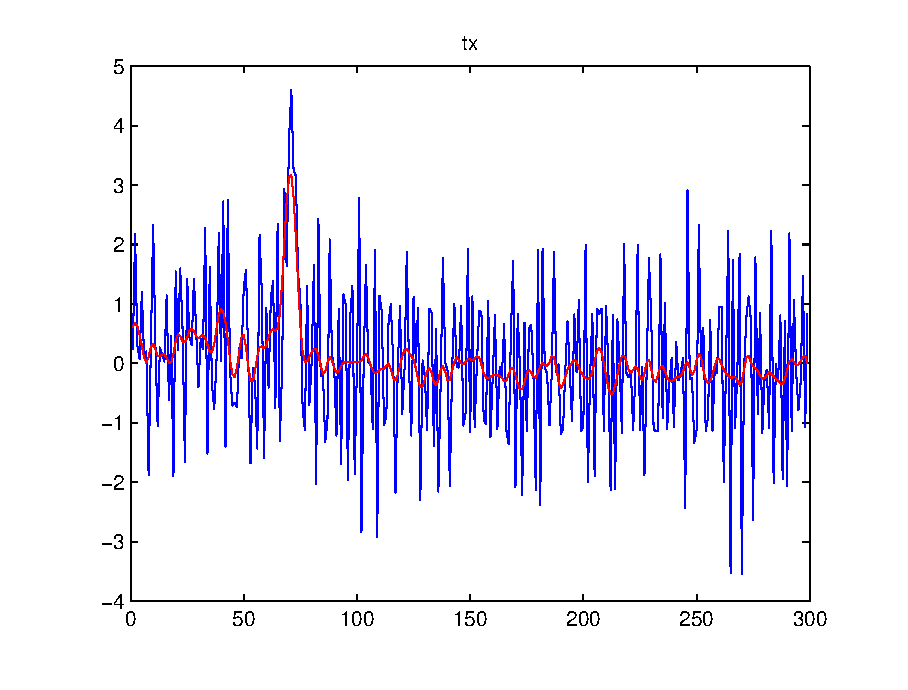
\includegraphics [width=3.5in]{tx.eps}
			\caption{ $H_i(1,3)$ vs $i$}
		\end{figure}
		\begin{figure}[h]
			\centering
			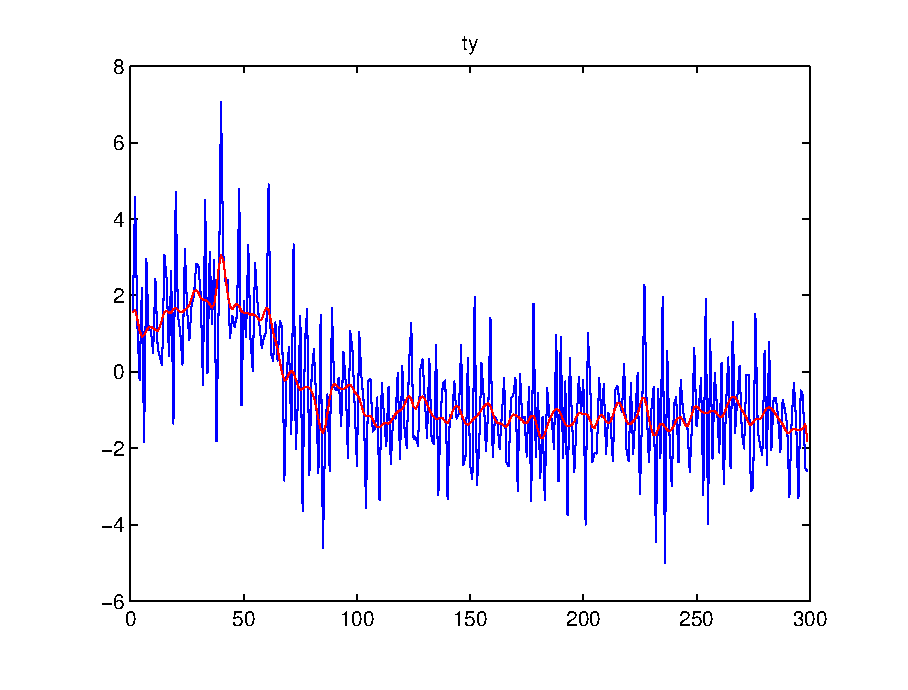
\includegraphics [width=3.5in]{ty.eps}
			\caption{ $H_i(2,3)$ vs $i$}
		\end{figure}
\end{itemize}



\item Now given the smoothed sequence, re-warp the different frames of the shaky video to generate a more stable version of the video. (My hunch is that most of you will find this part to be trickier than what is may initially appear!). View the shaky and stabilized videos together by (1) putting them in a single array of size $2H \times W \times T$ where $(H,W)$ is the size of each frame and $T$ is the number of frames, and (2) using the routine `displayvideo' mentioned earlier.  Also your MATLAB program should write the combined video to a file and give it a logical name that you print on screen. \textsf{[5 points for successfully dealing with 2D translation + 3 points for rotation + 2 BONUS points for the affine case]}
\begin{itemize}
	\item[Ans.] For resulting videos, please look in the folder 'video stabilization'.	
\end{itemize}
	
\item After patting yourself on the back for your hard work :-), it's now time to act as your own critic: What are the limitations of what you have developed? For example, can you think of certain types of videos or motion models or other situations your program is or will be unable to handle? \textsf{[3 points]}

\begin{itemize}
	\item[Ans.] If the underlying motion of the video can't be explained by a homography, our method fails badly. An example can be seen in last few frames of 'gbus.avi'. Here, different vehicles move at different speeds making it impossible to be explained by a homography.
\end{itemize}

\end{itemize}


\end{enumerate}



\end{document}